\renewcommand{\inputfile}{\version\ - Predrag edited 2009-08-18 slice.tex}
% siminos/thesis/chapters/slice.tex
% $Author$ $Date$

% Predrag                           Aug 18 2009
%       extracted from wilczak/blog/flow.tex




\PCedit{
\subsection{$\SOn{2}$ equivariance}

\CLf\ \refeq{eq:CLeR} is equivariant,
$v(\ssp)= g^{-1} v(g \ssp)$,
under
$\SOn{2}$ rotations \refeq{eq:RotCLe5d} induced by the Lie algebra generator
  \beq
 \Lg =   \left(\barr{ccccc}
    0  &  1 & 0  &  0 & 0  \\
   -1  &  0 & 0  &  0 & 0 \\
    0  &  0 & 0  &  1 & 0  \\
    0  &  0 &-1  &  0 & 0 \\
    0  &  0 & 0  &  0 & 0
    \earr\right)
 \,.
 \label{ZMgen}
 \eeq
Using a 2\dmn\ matrix representation of an $\SOn{2}$ rotation by a
finite angle $\theta$,
    \PC{is the sign standard?}
\beq
 {\bf R}(\theta) = e^{i\Lg \theta}
 = \cos\theta
   \left(\barr{cc}
    1  &  0   \\
    0  &  1
    \earr\right)
 + \sin\theta
   \left(\barr{cc}
    0  &  1   \\
   -1  &  0
    \earr\right)
 =   \left(\barr{cc}
    \cos\theta  &  \sin\theta   \\
   -\sin\theta  &  \cos\theta
    \earr\right)
 \,,
\label{2Drotation}
\eeq
%  $0  \leq \theta < \pi/2$.
we can express the action of an $\SOn{2}$ group element
${D}(\theta)$ as a simultaneous finite rotation in the $(x_1,x_2)$
and $(y_1,y_2)$ planes:
\beq
 {D}(\theta) = e^{i\Lg\theta}
 =   \left(\barr{ccc}
    {\bf R}(\theta) &  0              & 0  \\
    0               & {\bf R}(\theta) & 0  \\
    0               &  0              & 1
    \earr\right)
% =   \left(\barr{ccccc}
%    \cos\theta  &  \sin\theta & 0  &  0 & 0  \\
%   -\sin\theta  &  \cos\theta & 0  &  0 & 0 \\
%    0  &  0 & \cos\theta  &  \sin\theta & 0  \\
%    0  &  0 &-\sin\theta  &  \cos\theta & 0 \\
%    0  &  0 & 0  &  0 & 1
%    \earr\right)
 \,.
 \label{ZMrotation}
 \eeq
% $\SOn{2}$ is a commutative, Abelian group.
The infinitesimal statement of invariance is obtained by
expanding $g=e^{i\Lg_a \theta_a}$ for small $\theta_a$ and
keeping the leading $\theta_a$ term in $v(\ssp)= g^{-1} v(g \ssp)$:
    \PC{ This general discussion belong to
    \refchap{chap:Symmetry}, as the second, infinitesimal
    rotations part of \refsect{sec:symIntro} (where the first
    part is the statement of equivariance under global
    rotations). Checking equivariance as a condition on Lie algebra
    is much easier than checking it for global, finite angle rotations,
    especially for non-trivial Lie groups.}
\beq
  \left(
    \Lg_a  - (\Lg_a \ssp) \cdot \frac{\partial}{\partial \ssp}
  \right) v(\ssp) =
  (\Lg_a)_{ij} v_j(\ssp) - \Mvar_{ik} (\Lg_a)_{kj} \ssp_j =0
  \,,
\ee{inftmInv}
where the \stabmat\ for \CLf\ \refeq{eq:CLeR} is given by
  \beq
\Mvar =
  \left(\barr{ccccc}
    -\sigma    	& 0 		& \sigma & 0    &  0 \\
	0 	& -\sigma       & 0      & \sigma   &  0 \\
	\RerCLor-z  &     -\ImrCLor      & -1     & -e & -x_1 \\
	\ImrCLor     & \RerCLor-z       	& e  	& -1       & -x_2 \\
	y_1     & y_2           & x_1    & x_2      & -b
    \earr\right)
\,.
  \ee{CLeStabMat}

\PublicPrivate{}{
\PCedit{
$  {\cal L}_g v(x) = \left(\Lg_a  - (\Lg_a \ssp) \cdot
\frac{\partial}{\partial \ssp} \right) v(\ssp) $ is the {\em
Lie derivative} of the flow $v$ with respect to the direction
of the group-rotation induced flow $\Lg_a \ssp$.
\refeq{inftmInv} is the {\em Lie bracket} (called the {\em
Poisson bracket} by Arnol'd\rf{arnold89}) of the two flows.
The Lie derivative $  {\cal L}_g v$ measures how much the
flows induced by the two vector fields commute with each
other. The commute if and only if their Lie bracket is equal
to zero, as is the case in \refeq{inftmInv}.
}
}% end \PublicPrivate

Next we decompose $\vf(x)$
in \refeq{eq:difeq} in a part $\vf_\shortparallel$ parallel
to the group action and a part $\vf_\perp$ transverse to it,
\beq
	\vf(\ssp)=\vf_\shortparallel(\ssp)+\vf_\perp(\ssp)\,,
\ee{flowSplit}
using the projection operator
\beq
 	\PperpOp_{ij}(\ssp)=\delta_{ij}-
    \frac{(\Lg \ssp)_i (\Lg \ssp)_j}{(\Lg \ssp)^2}
\ee{transvProj}
that projects a $d$-dimensional flow $\vf(\ssp)$ onto
flow
\beq
	\dot{\ssp}_\perp = \vf_\perp(\ssp) = \vf(\ssp)
    - \Lg \ssp \frac{(\Lg\ssp)\cdot\vf(\ssp)}{(\Lg \ssp)^2}
\ee{transvFlow}
in a $(d\!-\!1)$-dimensional {\csection} transverse to the
direction fixed by the point $\ssp$.
By ignoring
the flow component that can be compensated for by an
$\SOn{2}$ rotation we quotient the flow by $\SOn{2}$. The
idea is presumably very old; for example, it is stated as the
problem 1. of Sect. 6.2 of Arnol'd {\em Ordinary Differential
Equations}\rf{arnold92}. Note, however, that a choice of
$\ssp_0$ fixes only a direction, so the reduced flow is still
equivariant under the action of discrete cyclic group $\Ztwo
= \{e,D(\pi)\}$ on $\ssp$, $\vf(\ssp)$ and the reference
point $\ssp_0$, just as was the case \refeq{LorenzR} for the
Lorenz flow \refeq{Lorenz}.
    \PC{\emph{Mea culpa}: Here I screwed up. I forgot that rotation
    moves $v$ and counter-moves $\ssp$ in $v(\ssp)$, \ie,
    acts by the Lie derivative \refeq{inftmInv}. I could never
    understand why we do not see a translational zero eigenvalue
    everywhere (the Lie group acts globally and commutatively
    right?), but only on \eqva, \reqva\ and \rpo s. Presumably
    the projection operator \refeq{transvProj} is OK for the
    \reqv\ calculation of \refeq{sect:StabEq},
    as the action of the group on $\ssp_{\REQB{1}}$ is trivial?
    Not sure how to rewrite the decomposition induced by
    \refeq{transvProj} correctly, in
    terms of the full Lie derivative action, and not only the $\Lg$
    action.
    }
}%end \PCedit



\section{\Reducedsp}
\label{sect:reducedStateSp}


\subsection{Method of moving frames, finite time steps}
\label{sect:MovFrame}
% Predrag                           Jul 19 2009
% Predrag                           Aug 12 2009

In refsect?? we have discussed symmetry reduction by the
method of {\em moving frames} of Cartan\rf{CartanMF}, in the
formulation of Fels and
Olver\rf{FelsOlver98,FelsOlver99,OlverInv}.
The moving frames method allows the determination of (non-polynomial)
invariants of the group action by a simple and efficient
algorithm that works well in high-dimensional \statesp s.
    \PC{Vaggelis, add references here? {\bf ES}: mmm... SiminosThesis?}
    \PC{Vaggelis, why ``(non-polynomial)'' invariants?
        length$^2$ is polynomial {\bf ES}: It is the only one though.
        {\bf PC}: is this an answer?}

As far as we are aware,
our exposition does not follow the above references.

Split up the integration of the $\SOn{2}$-equivariant ODE into
a sequence of short time steps, each followed by a rotation
such that the next segment initial point is in the point
$\ssp^{*}$ {\slice}, a $(d\!-\!1)$-dimensional hyperplane
normal to the group rotation tangent $t^{*}$ at point
$\ssp^{*}$:
\beq
(\ssp- \ssp^{*}) \cdot t^{*}=0
    \,,\qquad
t^{*} = \Lg \cdot \ssp^{*}
\,.
\ee{PCsectQ}
For any $\hat{\ssp}$, $\ssp =
\mathbb{G}(\theta)\cdot\hat{\ssp}$ is defined to be the
rotation of $\hat{\ssp}$ that lies in the \slice. Such a
map from a point in space to the group action is called a
\emph{moving frame} in the formulation of Fels and
Olver\rf{FelsOlver98,FelsOlver99,OlverInv}. A generic point
$\ssp^{*}$ not on the $z$ axis should suffice to fix a good
\slice, for example a point on an \reqv\ group orbit,
$\ssp^{*} = \ssp_{\REQB{}1}$.
As $\ssp^{*} \cdot t^{*}=0$ by the antisymmetry of
$\Lg$, \refeq{PCsectQ} reduces to the condition
\beq
0 = \ssp \cdot \Lg \cdot \ssp^{*}
  %= \mathbb{G}(\theta) \cdot \hat{\ssp}   \cdot \Lg \cdot \ssp^{*}
	=\hat{\ssp} \cdot \mathbb{G}(\theta)^T \cdot \Lg \cdot \ssp^{*}
\ee{PCsectQ1}
that determines $\theta$ for a given $\hat{\ssp}$. Each
circle intersects the section exactly twice,  so there are
two solutions, separated by $\pi$. We select the one
with a smaller clockwise rotation angle into the \slice.
The $z$-axis invariant subspace is always within the section,
so this is a nice, globally transverse \slice.

%%%%%%%%%%%%%%%%%%%%%%%%%%%%%%%%%%%%%%%%%%%%%%%%%%
% computed by PCunrot.nb
\SFIG{PCunrot}
{}{
Method of moving frames, finite time steps version: a
trajectory started on the \slice, with $\ssp_1^{(0)}
=0$, evolves for a finite time to a \statesp\ point with a
non-zero $\hat{\ssp}_1^{(1)}$. The {\em entire} \statesp\ is then
rotated (the `frame is moved') so that the equivalent point
on the circle lies on the \slice, $\ssp_1^{(1)} =0$.
Thus after every finite time step followed by a rotation the
trajectory returns to the 4$\dmn$ $\ssp_1 =0$
\reducedsp.
}
{fig:PCunrot}
%%%%%%%%%%%%%%%%%%%%%%%%%%%%%%%%%%%%%%%%%%%%%%%%%%

    \PC{generate quality PCunrot.eps from PCunrot.nb}
\refFig{fig:PCunrot} illustrates the method of moving frames,
finite time version, for a \slice\ motivated by the polar
form of the \CLe\ of \refsect{sect:coordChange}. It is
defined, for example, by taking
$(x^{*}_1,x^{*}_2,y_1^{*},y_2^{*})=(0,1,0,0)$,
$x_1=0,\,x_2>0$. Start at $\ssp^{(0)}$ with $\ssp_1^{(0)}
=0$, evolve for a finite time to $\hat{\ssp}^{(1)}$. Compute
the polar angle $\theta_1$ of $\hat{\ssp}^{(1)}_1$ in the
$(\ssp_1,\ssp_2)$ plane, and rotate the {\em entire}
\statesp\ (hence `moving frame') clockwise by $\theta_1$,
$\ssp^{(1)} = \mathbb{G}(\theta_1) \cdot \hat{\ssp}^{(1)}$,
to satisfy the $\ssp_1=0$ \slice\ condition. Repeat. The
trajectory remains in the 4$\dmn$ $\ssp_1=0$
\reducedsp.
    \PC{complete \refFig{fig:PCunrot}
        - need to draw a longer segment of the initial trajectory,
        to make it clearer that the whole segment is rotated.
       }

\subsection{Method of moving frames, differential formulation}
\label{sect:MovFrameODE}

% Predrag, Vaggelis                         Aug 13 2009
%           fixed the details as suggested
% Vaggelis                                  Aug 12 2009
%           \refeq{EqMotionMovFramePC} is correct
%           there are problems with the derivation.


\begin{bartlett}
I made a wrong mistake.
\bauthor{Yogi Berra}
\end{bartlett}

\noindent
Infinitesimal time version of the moving frames symmetry
reduction is attained by taking small time steps in
\reffig{fig:PCunrot} and dropping the higher order terms, as
in \refsect{sect:SymmDyn}. For infinitesimal  $d\theta$ we
set $\sin d\theta \approx d\theta$, $\cos d\theta \approx
1$, $\mathbb{G}(d\theta) \approx {1}+ d\theta \, \Lg $, and
the condition \refeq{PCsectQ} for rotating an infinitesimal
time evolution step $dx = v\,dt$ back into the \slice\
\[
0 = (\ssp + dx) \cdot \mathbb{G}(d\theta)^T \cdot \Lg \cdot \ssp^{*}
  \approx (\ssp + dt\,v) \cdot (1+ d\theta\,\Lg)^T \cdot \Lg \cdot \ssp^{*}
  \approx dt\,v \cdot \Lg \cdot \ssp^{*} - d\theta\,\ssp \cdot \Lg \cdot \Lg \cdot \ssp^{*}
\]
%\ES{It is $\Lg^T=-\Lg$.}
yields
        \PC{will need quality infMF.eps}
\beq
d\theta \approx \frac{v \cdot \Lg \cdot \ssp^{*}}
                     { \ssp \cdot \Lg \cdot \Lg \cdot \ssp^{*}} \,  dt
\,.
\ee{MFdtheta}

%%%%%%%%%%%%%%%%%%%%%%%%%%%%%%%%%%%%%%%%%%%%%%%%%%
% File: infMF.xfig
\SFIG{infMF}
{}{
Method of moving frames, infinitesimal formulation.
}
{fig:infMF}
%%%%%%%%%%%%%%%%%%%%%%%%%%%%%%%%%%%%%%%%%%%%%%%%%%

Let $u(\ssp)$ be the vector field that generates the flow in
the \reducedsp. According to \reffig{fig:infMF}, in
the limit that $\mathbb{G}(d\theta) \approx 1+d\theta\,\Lg$ the
infinitesimal time step under $u$ is connected to the time
step under $v$ by
    \PC{in \reffig{fig:infMF}:\\
        * Change $R$ into $\mathbb{G}$. \\
        * Draw $z$ axis
        (would lie horizontal in the present version, so tilt the figure).\\
        * Indicate $d\theta$ by drawing from origin, spanned by arc $x, x+v dt$.\\
        * Include a segment of the group-orbit ellipse, so $t^{*}$ is
          clearly visualized as a tangent.\\
        * Add arrows to $v dt$, $u dt$.
        }
\[
 \ssp+u\,dt=  (1+d\theta\Lg)\cdot(\ssp+v dt)\,.
\]
Dropping second order terms, dividing through with $dt$
\[
 u = v+\frac{d\theta}{dt} \,\Lg\cdot\hat{x}
 \,,
\]
and substituting \refeq{MFdtheta} gives the \reducedsp\ equations:
\beq
\dot{\ssp} = v - \frac{(v \cdot \Lg \cdot \ssp^{*})}{(\ssp \cdot\ssp^{*})_4}
                 \, \Lg \cdot \ssp
\,,
\ee{EqMotionMovFramePC}
where we have used the fact that
$- \ssp \cdot \Lg\cdot\Lg \cdot \ssp^{*}
 = (\ssp \cdot \ssp^{*})_4 =
    x_1 x_1^{*}
   +x_2 x_2^{*}
   +y_1 y_1^{*}
   +y_2 y_2^{*}
$
is the dot-product restricted to the 4-dimensional
representation of $\SOn{2}$. By construction, the motion
stays in the $(d\!-\!1)$-dimensional \slice.

    \PC{
A more elegant derivation is given in
\refrefs{rowley_reconstruction_2000,rowley_reduction_2003}.
By equivariance on can always write the full \statesp\ trajectory
as $\ssp(t)= \mathbb{G}(t)\cdot\sspRed(t)$, where the \reducedsp\
trajectory $\sspRed(t)$ is to be fixed by some condition, and $\mathbb{G}(t)$
is the group action that rotates  $\ssp$ into $\sspRed$ at time $t$. The time
derivative is then
$\dot{\ssp}= \vel(\mathbb{G}\sspRed) = \dot{\mathbb{G}}\sspRed + \mathbb{G}\velRed$,
where the \reducedsp\ velocity fields is $\velRed=\dot{\sspRed}$. This leads to
the \reducedsp\ flow
\[
\velRed(\sspRed) = \vel(\sspRed) - \mathbb{G}^{-1} \dot{\mathbb{G}} \, \sspRed
\,.
\]
    }
A generic  $ \ssp^{*}$ can be brought to form $ \ssp^{*} =
(0,1,y_1^{*},y_2^{*})$ by a rotation and rescaling. Then $\Lg
\cdot \ssp^{*}  = (1,0,y_2^{*},-y_1^{*})$, and
\beq
\frac{(v \cdot \Lg \cdot \ssp^{*})}{(\ssp \cdot\ssp^{*})_4} =
\frac{v_1 + v_3 y^{*}_2 -v_4 y^{*}_1}
     {x_2 + y_1 y^{*}_1 + y_2 y^{*}_2}
%\frac{v_1 x^{*}_2 -v_2 x^{*}_1 + v_3 y^{*}_2 -v_4 y^{*}_1}
%     {v_1 x^{*}_1 + v_2 x^{*}_2 + v_3 y^{*}_1 + v_4 y^{*}_2}
\,.
\label{PCsectSin}
\eeq

%
%%%%%%%%%%%%%%%%%%%%%%%%%%%%%%%%%%%%%%%%%%%%%%%%%%%%%%%%%%%%%%%%%%
% CLEpcSect.png computed by  CLEfinal.nb (repo: vaggelis)
% CLEpcSect2.png computed by CLEfinal.nb (repo: vaggelis)
\begin{figure}[ht]
\begin{center}
(a) 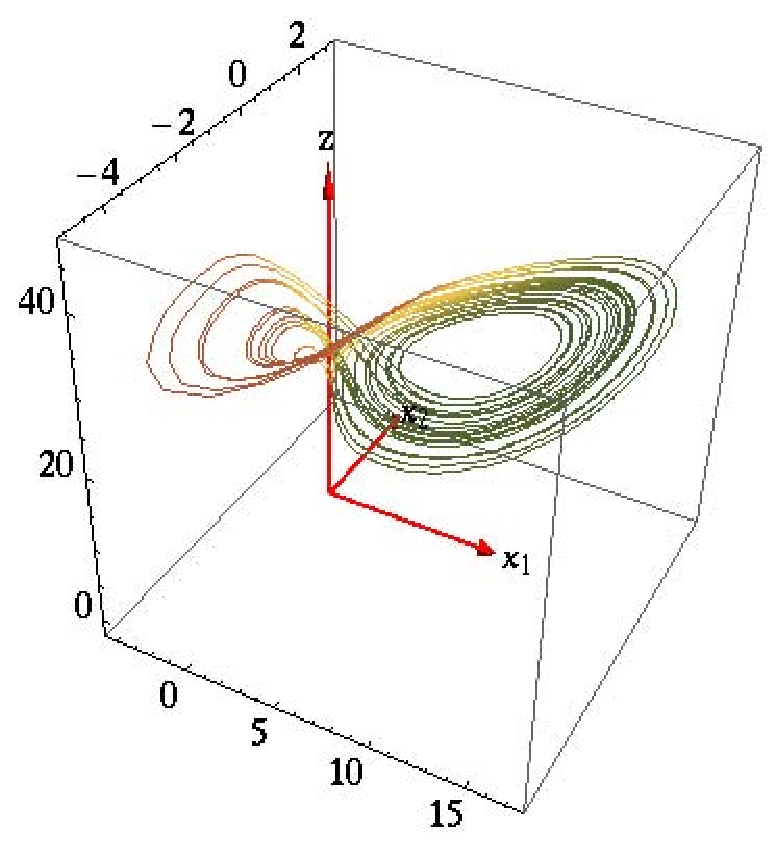
\includegraphics[width=0.40\textwidth]{../figs/CLEpcSect}
(b) 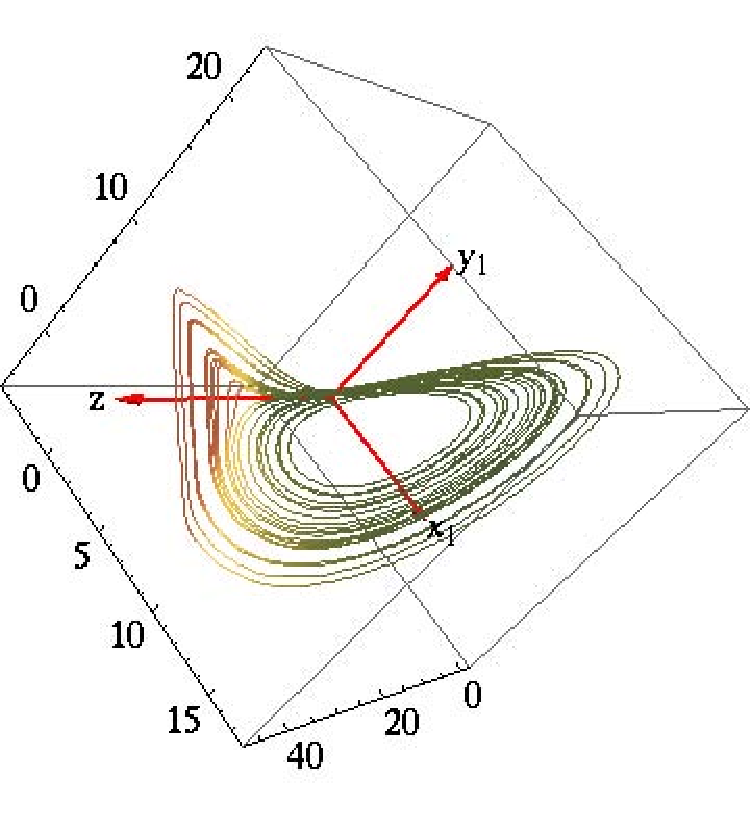
\includegraphics[width=0.43\textwidth]{../figs/CLEpcSect2}
\end{center}
\caption{
Method of moving frames, \slice\ fixed by a point on an
\reqv\ group orbit, $\ssp^{*} = \ssp_{\REQB{}1}$. The strange
attractor of \reffig{fig:CLEx1x2z} in the \reducedsp\
of \refeq{EqMotionMovFramePC}:
(a) $\{x_1,x_2,z\}$ projection,
(b) $\{x_1,y_1,z\}$ projection.
Color-coding indicates $(\hat{\ssp} \cdot \hat{\ssp^{*}})_4$
where $\hat{.}$ stands for unit vector, with green indicating values
of the inner product close to $1$ and brown indicating values
close to $0$.
    }
\label{fig:CLEpcSect}
\end{figure}
%%%%%%%%%%%%%%%%%%%%%%%%%%%%%%%%%%%%%%%%%%%%%%%%%%%%%%%%%%%%%%%%
%
    \PC{will need quality CLEpcSect.eps, CLEpcSect2.eps}
A long time trajectory of \refeq{EqMotionMovFramePC} with
$x^*$ on the \reqv\ \REQB{1} group orbit is shown in
\reffig{fig:CLEpcSect}.
\ES{I will add a scale in \reffig{fig:CLEpcSect} but it is too
late here to do it tonight.}
As initial condition
we chose an initial point on the unstable manifold
of \REQB{1}, rotated back to the \slice\ by angle $\theta$ as
prescribed by \refeq{PCsectQ1}. In \reffig{fig:CLEpcSect} we
show the part of the trajectory for $t\in\left[70,100\right]$.
The \reqv, now an equilibrium of the
\reducedsp\ dynamics, organizes the flow into a R\"ossler type
attractor. There appears to be no singularity in this
attractor although we can run into trouble with
\refeq{EqMotionMovFramePC} wherever the denominator in
\refeq{MFdtheta} vanishes, \ie, the direction of group
action on the point $\ssp$ is perpendicular to the direction
of group action on $\ssp^*$.
\ES{dropped but we need to discuss:
Apparent lack of singularities in \reffig{fig:CLEpcSect} appears
fortuitous or perhaps even a programming error.
This is a 4\dmn\ subspace, and indeed our simulations encounter
this subspace very quickly, with \reducedsp\ velocity going off to infinity.
For example, for
$\ssp^* \approx  \ssp_{\REQB{}1} = (8.48,0.077,8.48,0,26.99)$
on \reqv\ \REQB{1} group orbit,
and initial point
$\ssp(0) \approx  (4.81,0.154,7.59,0.281,15.9)$
      taken from a long run on the strange attractor, the denominator
$(\ssp(t) \cdot\ssp^{*})_4$ vanishes at $t \approx 1.217\cdots$.
    } %end ES
%    \ES{Could this happen for the present group action and
%    choice of \slice? {\bf PC:} seems yes...}
    \PC{ in \reffig{fig:CLEpcSect}:\\
        * Mark $\ssp_{\REQB{}1}$ \\
        * Draw stable eigenvector of $\ssp_{\REQB{}1}$\\
        * State value of $\ssp_{\REQB{}1}$ somewhere
        }


%%%%%%%%%%%%%%%%%%%%%%%%%%%%%%%%%%%%%%%%%%%%%%%%%%
% computed by PCunrot.nb
\SFIG{PCunrot1}
{}{
Method of moving frames, continuous time version, for the
polar coordinates motivated $x^{*}=(0,1,0,0)$,
$x_1=0,\;x_2>0$, \slice. The strange attractor of
\reffig{fig:CLEx1x2z} in the \reducedsp,
$\{x_2,y_2,z\}$ projection exhibits a discontinuity at
$x_2=0$.
}
{fig:PCunrot1}
%%%%%%%%%%%%%%%%%%%%%%%%%%%%%%%%%%%%%%%%%%%%%%%%%%

Indeed, the method does encounter singularities in
subsets of \statesp.
For example, the \reducedsp\ equations \refeq{PCsectSin}
for the polar coordinates inspired \slice\
$x^{*}=(0,1,0,0)$, $x_1=0,\;x_2>0$,
%this is illustrated by \reffig{fig:PCunrot}.
%$(\rho_1,\theta_1)$ are polar coordinates, $\rho_1 =
%\sqrt{\ssp_1^{ 2} + \ssp_2^{2}}$, see \refeq{eq:CartToPol},
are given by
\beq
\dot{\ssp} = v - \frac{v_1}{\ssp_2} \Lg \cdot \ssp
\,.
\ee{EqMotionMovFrame}
A typical trajectory is shown in \reffig{fig:PCunrot1}.
The problem with defining the \slice\ by
\refeq{EqMotionMovFrame} is apparently that it fixes rotations
in the $(\ssp_1,\ssp_2)$ plane, not the full 4\dmn\ space.
